Eksperimenteringen er utført på en Macbook Air med 1.8 GHz Intel Core i7 prosessor og 4 GB 1333 MHz DDR3 minne. Det er totalt sett 160 benchmarksett som implementasjonene er evaluert på. Hvor mange det ble funnet en løsning på varierte avhengig av om tilleggsressursene var med eller ikke og tidsgrensen som var satt.

\begin{table}[!h]
\caption{Relativ optimalitets indeks $w_{rq}$ for de forskjellige modellene med tidsgrense på 100 sekunder}
\begin{center}
\begin{tabular}{ | c | c | c | c | c | c | c | c | c | c | c | }
\hline
\textbf{Modell} & \multicolumn{4}{|c|}{\textbf{2 kraner}} & \multicolumn{4}{|c|}{\textbf{3 kraner}} & \multicolumn{2}{|c|}{\textbf{Alle}} \\ \hline
$\sharp Act(\sharp P)$ & \multicolumn{2}{|c|}{$< 100 (25)$} & \multicolumn{2}{|c|}{$\ge 100 (55)$} & \multicolumn{2}{|c|}{$< 100 (25)$} & \multicolumn{2}{|c|}{$\ge 100 (55)$} & \multicolumn{2}{|c|}{(160)} \\ 
\hline
Modell & $w_{rq}$ & $\%^{(1)}$ & $w_{rq}$ & $\%^{(1)}$  & $w_{rq}$ & $\%^{(1)}$ & $w_{rq}$ & $\%^{(1)}$ & $w_{rq}$ & $\%^{(1)}$ \\ \hline
$LS1 \sharp 1\sharp 3$ & 1.578 & 100 & 1.905 & 100 & 1.593 & 100 & 1.731 & 100 & 1.745 & 100 \\
$LS1 \sharp 2\sharp 3$ & 1.672 & 100 & 1.961 & 100 & 1.711 & 100 & 1.766 & 100 & 1.810 & 100 \\
$LS2 \sharp 1\sharp 3$ & 1.144 & 84 & 1.160 & 27.3 & 1.157 & 68 & 1.042 & 10.91 & 1.142 & 36.88 \\
$LS2 \sharp 2\sharp 3$ & 1.256 & 76 & 1.313 & 30.91 & 1.243 & 72 & 1.041 & 18.18 & 1.232 & 40 \\
$LS2 \sharp 1\sharp 4$ & 1.031 & 100 & 1.002 & 100 & 1.023 & 100 & 1.003 & 100 & 1.010 & 100 \\
\hline
\multicolumn{11}{l}{\begin{minipage}{6in}$^{(1)}$ prosentandel løste probleminstanser\newline
$\sharp 1$ er løsninger uten varmebegrensning\newline
$\sharp 2$ er løsninger med varmebegrensning \newline
$\sharp 3$ er løsninger med sikkerhetsbegrensning \newline
$\sharp 4$ er løsninger uten sikkerhetsbegrensning\end{minipage}}
\end{tabular}
\end{center}
\label{tab:resultaterSum100s}
\end{table}

\begin{table}[!h]
\caption{Relativ optimalitets indeks $w_{rq}$ for de forskjellige modellene med tidsgrense på 5 sekunder}
\begin{center}
\begin{tabular}{ | c | c | c | c | c | c | c | c | c | c | c | }
\hline
\textbf{Modell} & \multicolumn{4}{|c|}{\textbf{2 kraner}} & \multicolumn{4}{|c|}{\textbf{3 kraner}} & \multicolumn{2}{|c|}{\textbf{Alle}} \\ \hline
$\sharp Act(\sharp P)$ & \multicolumn{2}{|c|}{$< 100 (25)$} & \multicolumn{2}{|c|}{$\ge 100 (55)$} & \multicolumn{2}{|c|}{$< 100 (25)$} & \multicolumn{2}{|c|}{$\ge 100 (55)$} & \multicolumn{2}{|c|}{(160)} \\ 
\hline
Modell & $w_{rq}$ & $\%^{(1)}$ & $w_{rq}$ & $\%^{(1)}$  & $w_{rq}$ & $\%^{(1)}$ & $w_{rq}$ & $\%^{(1)}$ & $w_{rq}$ & $\%^{(1)}$ \\ \hline
$LS1 \sharp 1\sharp 3$ & 1.585 & 100 & 1.907 & 91 & 1.608 & 100 & 1.731 & 91 & 1.745 & 94 \\
$LS1 \sharp 2\sharp 3$ & 1.674 & 100 & 1.963 & 91 & 1.718 & 100 & 1.767 & 91 & 1.808 & 94 \\
$LS1 \sharp 1\sharp 4$ & 1.031 & 100 & 1.003 & 91 & 1.023 & 100 & 1.004 & 91 & 1.011 & 94 \\
$LS1 \sharp 2\sharp 4$ & 1.074 & 100 & 1.020 & 91 & 1.064 & 100 & 1.013 & 91 & 1.034 & 94 \\
$LS2 \sharp 1\sharp 3$ & 1.155 & 84 & 1.160 & 25 & 1.323 & 60 & 1.060 & 9 & 1.151 & 36 \\
$LS2 \sharp 2\sharp 3$ & 1.245 & 84 & 1.288 & 24 & 1.385 & 60 & 1.046 & 15 & 1.221 & 37 \\
$LS2 \sharp 1\sharp 4$ & 1.031 & 100 & 1.003 & 91 & 1.023 & 100 & 1.004 & 91 & 1.011 & 94 \\
$LS2 \sharp 2\sharp 4$ & 1.074 & 100 & 1.020 & 91 & 1.064 & 100 & 1.013 & 91 & 1.034 & 94 \\
\hline
\multicolumn{11}{l}{\begin{minipage}{6in}$^{(1)}$ prosentandel løste probleminstanser\newline
$\sharp 1$ er løsninger uten varmebegrensning\newline
$\sharp 2$ er løsninger med varmebegrensning \newline
$\sharp 3$ er løsninger med sikkerhetsbegrensning \newline
$\sharp 4$ er løsninger uten sikkerhetsbegrensning\end{minipage}}
\end{tabular}
\end{center}
\label{tab:resultaterSum5s}
\end{table}

En måling av relativ kvalitet er brukt for å evaluere resultatene fra forskjellige strategier. Den avledede variabelen $w_{rq}$ er gitt ved (\ref{eq:relativkvalitet}).
\begin{equation}
w_{rq} = \frac{1}{| P_{sol} |} \sum_{P \in P_{sol}} \frac{w_{ms}(P)}{c_{lb,ms}(P)}
\label{eq:relativkvalitet}
\end{equation}
$P_{sol}$ er det settet med probleminstanser som er løst ved hver enkelt løsningsstrategi. Verdiene av $P_{sol}$ varierer fra løsningsstrategi til løsningsstrategi og disse gjennomsnittene er derfor ikke helt sammenlignbare, men de vil gi en indikasjon på kvaliteten på løsningen. $w_{rq}$ skiller ikke på strategier som feiler med å finne løsninger, men hvor robust løsningen er vil antallet løste probleminstanser indikere. Resultatene er summert opp i tabell \ref{tab:resultaterSum100s} og i tabell \ref{tab:resultaterSum5s}. Tabell \ref{tab:resultaterSum5s} viser at 5 sekunders kjøringer også gir relevante løsninger for samme kjøringer som er gjort i tabell \ref{tab:resultaterSum100s}. Det er kjørt noen ytterligere modeller i tabell \ref{tab:resultaterSum5s}.

Det kan finnes en annen teoretisk nedregrense da det her er valgt teoretisk nedregrense basert på det mest begrensede mannskap. Men i og med den er beregnet ut fra den mest begrensede ressursen er det fornuftig benchmark å sammenligne løsningene med denne.

En praktisk forståelse av denne prosjektoppgavens innføring av varmebegrensning er at teoretisk nødvendigvis må være $\ge$ teoretisk nedregrense uten varmebegrensning. Da teoretisk nedregrense i denne prosjektoppgaven er basert på mannskap, vil makespan ved innføring av varmebegrensning ser mer ugunstig ut. Om dette er en reell økning av teoretisk nedregrense eller er et resultat av dårlig optimalisering i løsningen pga. økning av kompleksitet, er vanskelig å avgjøre (dette er diskutert annet sted i prosjektoppgaven). Men en positiv praktisk konsekvens er at den planlagte løsningen med varmebegrensning er bedre da lokasjonen ikke får ressurser ut over sin begrensning.

\subsection{Uten varmebegrensning}
I tabell \ref{tab:resultaterSum100s} og \ref{tab:resultaterSum5s} er dette benevnt LS1 og 2 $\sharp 1$ $\sharp 3$ og $\sharp 4$ (dvs. med og uten sikkerhetsbegrensing).

LS1 løser alle probleminstanser og har en gjennomsnittlig makespan på 74.5\%. Makespan er for alle $Act(P)$ høye - i intervallet 57.8\%-90.5\%. Figur \ref{fig:RessursWithoutAct50Loc10Crew5Crane2LS1} viser at lokasjon 2 er fullt utnyttet. Kran 1 er på lokasjon 2 (fra probleminstansene). Ved å bruke søketid på 5 sekunder løser LS1 94\% av probleminstansene og har samme gjennomsnittlig makespan som med søketid på 100 sekunder, 74.5\%. Makespan er for alle $Act(P)$ høye - i intervallet 58.5\%-90.7\%.

LS2 løser i gjennomsnitt 36.9\% av probleminstansene og har makespan på 14.2\%. Makespan for alle $Act(P)$ varierer - i intervallet 4.2\%-15.7\%. Det laveste/høyeste resultatet er for henholdsvis 3 og 2 kraner $\ge 100(55)$. Dersom sikkerhetsbegrensningen fjernes i dette tilfellet reduseres makespan til intervall 2.3\%-0.3\% og alle probleminstanser løses. Figur \ref{fig:ResourceAct50Crane2LS2_UtenVarme_100s} viser at for det viste tilfellet er lokasjon 6 fullt utnyttet. Det er 2 kraner. Fordelingen av aktiviteter over tidsaksen er jevn. Med å bruke en søketid på 5 sekunder løser LS2 36\% av probleminstansene og har en gjennomsnittlig makespan på 15.1\%. Makespan for alle $Act(P)$ varierer - i intervallet 6.0\%-32.3\%.

Løsningene fra tabell \ref{tab:resultaterSum5s} med LS1 og LS2 uten sikkerhetsbegrensinger er identiske. Like mange probleminstanser er løst og gjennomsnittlig makespan verdi er også lik.

Tidene som Scheduler bruker for å finne løsninger på probleminstansene er sammenliggnet med å se på tidene for samme antall aktiviteter og henholdsvis to og tre kraner. Det er ingen klare skiller om probleminstansene inneholder to eller tre kraner. Tidene for å finne løsninger varierer fra 0 til over 100 sekunder, og det er ikke de probleminstansene med flest aktiviteter som bruker lengst tid. Tiden for å finne en løsning varierer også stort innenfor probleminstansene med samme antall aktiviteter.
\begin{figure}[!h]
\centering
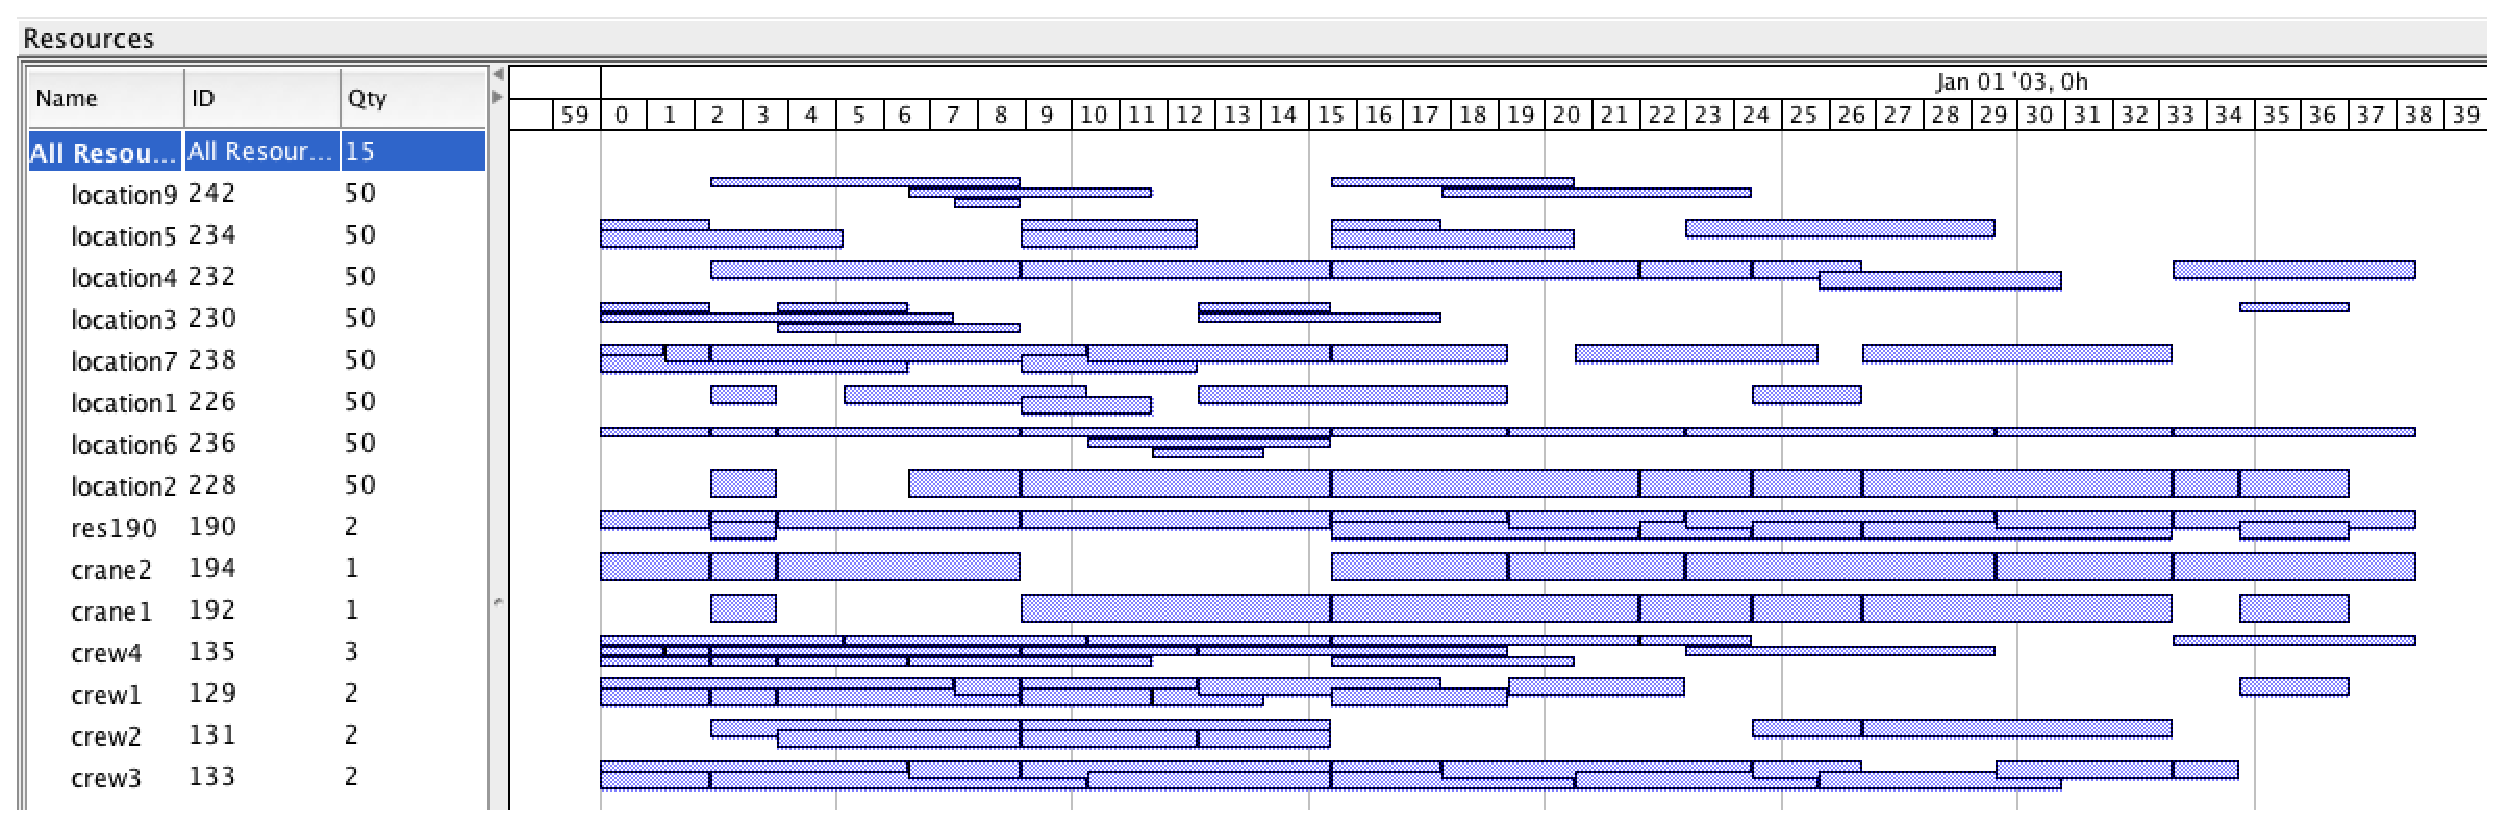
\includegraphics[scale=0.4]{content/gfx/ResourceAct50Crane2LS2_UtenVarme_100s}
\caption{Ressursskjema på Act50Loc10Crew5Crane2, LS2 og $\sharp1\sharp3$}
\label{fig:ResourceAct50Crane2LS2_UtenVarme_100s}
\end{figure}

\subsection{Med varmebegrensning}
I tabell \ref{tab:resultaterSum100s} og \ref{tab:resultaterSum5s} er dette benevnt LS1 og 2 $\sharp 2\sharp 3$ (dvs. med sikkerhetsbegrensing).

LS1 løser alle probleminstanser og har en gjennomsnittlig makespan på 81.0\%. Makespan er for alle $Act(P)$ høye - i intervallet 67.2\%-96.1\%. Figur \ref{fig:RessursWithAct50Loc10Crew5Crane2LS1} viser at for dette tilfellet er lokasjon 2 fullt utnyttet. Kran 1 er på lokasjon 2 (fra probleminstansene). Det er to kraner. Figur \ref{fig:RessursWithAct50Loc10Crew5Crane3LS1} viser at for det viste tilfellet er mannskap fullt utnyttet. Det er 3 kraner. Figur \ref{fig:GantWithAct50Loc10Crew5Crane2AssignHeat} med resultat for det viste tilfellet er vist som eksempel. Diagramet viser mange aktiviteter tidlig i planleggingen og få aktiviteter mot slutten. Tidsaksen viser en makespan på 57. Ved å benytte søketid på 5 sekunder løser LS1 94\% av probleminstansene og har en gjennomsnittlig makespan på 80.8\%. Makespan for alle $Act(P)$ høye - i intervallet 67.4\%-96.3\%.

LS2 løser i gjennomsnitt 40\% av probleminstansene og har makespan på 23.2\%. Makespan for alle $Act(P)$ er lave - i intervallet 4.1\%-31.3\%. Det laveste resultatet er for 3 kraner og $\ge 100(55)$. Figur \ref{fig:GantWithAct50Loc10Crew5Crane2TFHeat} med resultat for det viste tilfellet vises som eksempel. Diagrammet viser noe bedre fordeling av aktiviteter enn figur \ref{fig:GantWithAct50Loc10Crew5Crane2AssignHeat}. Tidsaksen viser en makespan på 48. Ved å benytte søketid på 5 sekunder løser LS2 37\% av probleminstansene med en gjennomsnittlig makespan på 22.1\%. Makespan for alle $Act(P)$ er lave - i intervallet 4.6\%-38.5\%.
\begin{figure}[!h]
\centering
\includegraphics[scale=0.25]{content/gfx/Act50Crane2GantAssignHeat}
\caption{Gantskjema på Act50Loc10Crew5Crane2 med varmebegrensning, LS1 og $\sharp2\sharp3$}
\label{fig:GantWithAct50Loc10Crew5Crane2AssignHeat}
\end{figure}
\begin{figure}[!h]
\centering
\includegraphics[scale=0.25]{content/gfx/Act50Crane2TimesForwardHeat}
\caption{Gantskjema på Act50Loc10Crew5Crane2 med varmebegrensning, LS2 og $\sharp2\sharp3$}
\label{fig:GantWithAct50Loc10Crew5Crane2TFHeat}
\end{figure}

Løsningene fra tabell \ref{tab:resultaterSum5s} med LS1 og LS2 uten sikkerhetsbegrensinger er identiske. Like mange probleminstanser er løst og gjennomsnittlig makespan verdi er også lik.

Tidene som Scheduler bruker for å finne løsninger på probleminstansene er sammenliggnet med å se på tidene for samme antall aktiviteter og henholdsvis to og tre kraner. Det er ingen klare skiller om probleminstansene inneholder to eller tre kraner. Tidene for å finne løsninger varierer fra 0 til over 100 sekunder, og det er ikke de probleminstansene med flest aktiviteter som bruker lengst tid. Tiden for å finne en løsning varierer også stort innenfor probleminstansene med samme antall aktiviteter.